%%
%% Copyright 2007, 2008, 2009 Elsevier Ltd
%%
%% This file is part of the 'Elsarticle Bundle'.
%% ---------------------------------------------
%%
%% It may be distributed under the conditions of the LaTeX Project Public
%% License, either version 1.2 of this license or (at your option) any
%% later version.  The latest version of this license is in
%%    http://www.latex-project.org/lppl.txt
%% and version 1.2 or later is part of all distributions of LaTeX
%% version 1999/12/01 or later.
%%
%% This template has been modified by Philip Blakely for
%% local distribution to students on the MPhil for Scientific
%% Computing course run at the University of Cambridge.
%%

%% Template article for Elsevier's document class `elsarticle'
%% with numbered style bibliographic references
%% SP 2008/03/01
%%
%%
%%
%% $Id: elsarticle-template-num.tex 4 2009-10-24 08:22:58Z rishi $
%%
%%
\documentclass[final,3p,times,twocolumn]{elsarticle}

%% Use the option review to obtain double line spacing
%% \documentclass[preprint,review,12pt]{elsarticle}

%% Use the options 1p,twocolumn; 3p; 3p,twocolumn; 5p; or 5p,twocolumn
%% for a journal layout:
%% \documentclass[final,1p,times]{elsarticle}
%% \documentclass[final,1p,times,twocolumn]{elsarticle}
%% \documentclass[final,3p,times]{elsarticle}
%% \documentclass[final,3p,times,twocolumn]{elsarticle}
%% \documentclass[final,5p,times]{elsarticle}
%% \documentclass[final,5p,times,twocolumn]{elsarticle}

%% if you use PostScript figures in your article
%% use the graphics package for simple commands
%% \usepackage{graphics}
%% or use the graphicx package for more complicated commands
\usepackage{graphicx}

%% or use the epsfig package if you prefer to use the old commands
\usepackage{epsfig}

%% The amssymb package provides various useful mathematical symbols
\usepackage{amssymb}
%% The amsthm package provides extended theorem environments
\usepackage{amsthm}
%% The amsmath package provides mathematical tools
\usepackage{amsmath}

%% The hyperref package allows the use of hyperlinked references and citations
\usepackage{hyperref}\hypersetup{
    colorlinks=true,
    linkcolor=blue,
    filecolor=magenta,      
    urlcolor=cyan,
    pdftitle={Overleaf Example},
    pdfpagemode=FullScreen,
    }

%% The lineno packages adds line numbers. Start line numbering with
%% \begin{linenumbers}, end it with \end{linenumbers}. Or switch it on
%% for the whole article with \linenumbers after \end{frontmatter}.
%% \usepackage{lineno}

%% natbib.sty is loaded by default. However, natbib options can be
%% provided with \biboptions{...} command. Following options are
%% valid:

%%   round  -  round parentheses are used (default)
%%   square -  square brackets are used   [option]
%%   curly  -  curly braces are used      {option}
%%   angle  -  angle brackets are used    <option>
%%   semicolon  -  multiple citations separated by semi-colon
%%   colon  - same as semicolon, an earlier confusion
%%   comma  -  separated by comma
%%   numbers-  selects numerical citations
%%   super  -  numerical citations as superscripts
%%   sort   -  sorts multiple citations according to order in ref. list
%%   sort&compress   -  like sort, but also compresses numerical citations
%%   compress - compresses without sorting
%%
%% \biboptions{comma,round}

% \biboptions{}


\journal{MPhil in Scientific Computing}

\begin{document}

\begin{frontmatter}

%% Title, authors and addresses

%% use the tnoteref command within \title for footnotes;
%% use the tnotetext command for the associated footnote;
%% use the fnref command within \author or \address for footnotes;
%% use the fntext command for the associated footnote;
%% use the corref command within \author for corresponding author footnotes;
%% use the cortext command for the associated footnote;
%% use the ead command for the email address,
%% and the form \ead[url] for the home page:
%%
%% \title{Title\tnoteref{label1}}
%% \tnotetext[label1]{}
%% \author{Name\corref{cor1}\fnref{label2}}
%% \ead{email address}
%% \ead[url]{home page}
%% \fntext[label2]{}
%% \cortext[cor1]{}
%% \address{Address\fnref{label3}}
%% \fntext[label3]{}

\title{Pressure-Velocity Coupling in the Incompressible Navier-Stokes equations with the SIMPLE algorithm}

%% use optional labels to link authors explicitly to addresses:
%% \author[label1,label2]{<author name>}
%% \address[label1]{<address>}
%% \address[label2]{<address>}

\author{BCN: 2023S1}

\address{Cavendish Laboratory, Department of Physics, J J Thomson
  Avenue, Cambridge. CB3 0HE}

\begin{abstract}
This MPhil assignment presents a numerical solver for the incompressible Navier-Stokes equations using the SIMPLE (Semi-Implicit Method for Pressure-Linked Equations) algorithm. The solver is developed using an unstructured finite-volume mesh class, which allows for the simulation of complex geometries with irregular boundaries.

The assignment provides an overview of the incompressible Navier-Stokes equations, the unstructured Finite-Volume method, and the SIMPLE algorithm, followed by a detailed explanation of the numerical implementation of the solver. The performance of the solver is evaluated by simulating a lid-driven cavity flow, which is solved implicitly using the standard discretization of the laplacian operator and an upwind differencing scheme for the convection term.

The results show that the solver accurately predicts the flow behaviour and the pressure distribution in the lid-driven cavity, and the pressure-velocity coupling is successfully resolved using the SIMPLE algorithm. The unstructured finite-volume mesh class allows for a high degree of flexibility in handling complex geometries, making the solver suitable for a wide range of fluid flow problems.

The study demonstrates the effectiveness of the SIMPLE algorithm and the unstructured finite-volume mesh class in solving incompressible flow problems. 
\end{abstract}

\end{frontmatter}

%%
%% Start line numbering here if you want
%%
% \linenumbers

%% main text
\section{Introduction}
To study practical, physically meaningful fluid flows using computer-based simulation, several pieces must come together, both mathematical and computational. The first is mathematical and dates back to the mid-eighteenth century with the derivation of the Euler equations, which were later unified into the more complete Navier-Stokes equations. In terms of describing fluid flows, this set of non-linear, partial differential equations (PDEs) provides a complete mathematical description of the physics of macroscale fluid flows involving neutrally charged microscale particles. However, analytical solutions to the equations are hard to come by and often too trivial for practical use. \\
The solution to this challenge is using numerical methods to transform partial differential equations into algebraic equations that can be solved computationally \cite{Moukalled2016TheMethod}. One such method is called the \textit{Finite Volume Method} and is a powerful technique for modelling fluid mechanics.

\subsection{The Finite Volume Method}
Fundamentally, the Navier-Stokes equations are a set of conservation laws, which are PDEs maintaining the following equality: the \textit{rate of change} of a specific quantity within a closed volume is equal to the \textit{net rate of flow} of the quantity through the surface of the volume \cite{Versteeg2007AnEdition}. \\
As mentioned above, the Finite Volume Method is a numerical technique that discretises both the volume-in-space of interest and the PDE used to describe the behaviour of the quantities within the volume. The method is a relatively recent development, appearing first in literature in the early 1970s \cite{McDonaldPW2015TheCascades}.
The spatial domain is discretised into a set of non-overlapping, arbitrarily shaped, polyhedral cells. Each face is shared by only two cells, and dependent variables are treated in a collocated arrangement, \cite{Rhie1982NumericalSeparation} \cite{Peric1985ADucts.}. \\ With geometric space in discrete form, the discretisation of the non-linear PDE remains. Many different methods exist, an extensive collection of which originate from the methods proposed by Crank \& Nicolson \cite{Crank1947AType}, Lax \cite{Lax1954WeakComputation} \cite{Lax1957HyperbolicII}, Lax \& Wendroff \cite{Lax1960SystemsLaws}, and notably, Godunov \cite{Godunov1959FiniteDynamics}. 

\subsection{The Incompressible Navier-Stokes Equations}
The importance of the Navier-Stokes equations in the study of fluid flows is once again stated, with simplifications of the equations providing necessary relief to the complexity allowing computational methods to be applied with relative ease. The full set of un-simplified equations in differential form reads as follows:

\begin{gather}
    \frac{\partial \rho}{\partial t} + \nabla \cdot (\rho \mathbf{v}) = 0 \label{eqn:NS_mass}
    \\ 
    \frac{\partial \rho \mathbf{v}}{\partial t} + \nabla \cdot [\rho \mathbf{v} \otimes \mathbf{v} + \mathbf{I}P] = \nabla \cdot \mathbf{\tau} + \rho \mathbf{f} \label{eqn:NS_momentum}
    \\
    \begin{split}
        \frac{\partial E}{\partial t} + \nabla \cdot [(E+P)\mathbf{v}] = \nabla \cdot (\kappa \nabla T) &+ \nabla \cdot (\mathbf{v \tau}) \\ &+ \rho \mathbf{f} \cdot \mathbf{v}
    \end{split}
    \label{eqn:NS_energy}
\end{gather}


See \ref{app:notation} for notational details. Equations (\ref{eqn:NS_mass}), (\ref{eqn:NS_momentum}), and (\ref{eqn:NS_energy})  represent the conservation of mass, momentum, and energy, respectively. All three are non-linear PDEs with temporal and spatial derivatives and source terms. \\ In this study, interest lies in studying steady-state incompressible fluid flows. This implies that the fluid is well approximated to have constant density, i.e. $\partial \rho / \partial t = 0$. The \textit{incompressible} limit of the Navier-Stokes equations then reduces to the simplified equations of the form:

\begin{gather}
\nabla \cdot \mathbf{v} = 0
\label{eqn:INS_mass} \\
\frac{\partial \mathbf{v}}{\partial t} + \nabla \cdot (\mathbf{v} \mathbf{v}) - \nabla \cdot (\nu \nabla \mathbf{v}) = -\nabla p + \mathbf{g}
\label{eqn:INS_momentum}
\end{gather}

Where $\rho$ is constant, allowing it to be removed from derivatives and divided through, $\nabla \cdot \mathbf{I} p$ simplifies to $ \nabla p$, $p=P/\rho$ is the kinematic pressure, the \textit{deviatoric stress tensor}, $\mathbf{\tau}=\nu \nabla \mathbf{v}$, with the kinematic viscosity, $\nu$, and the external force vector, $\textbf{f}$, is simply the force of gravity, $\mathbf{g}$. \\ 
Decoupling of pressure from density also results in the decoupling of the energy equation from the rest of the system; as a result, it is ignored for the purposes of this study. What remains is the momentum equation, which is non-linear in velocity and contains pressure-velocity coupling, which is the crux of the matter. Furthermore, the continuity equation (\ref{eqn:INS_mass}) enforces a divergence-free velocity field constraint on the system. \\ The system can be solved either \textit{implicitly} or \textit{explicitly}. The difference lies in the method used to update the solution; the explicit method integrates the PDE over solutions from previous times ($t$, $t - \Delta t$) and uses these to define the solution at a new time ($t+\Delta t$). This is a powerful technique and is used extensively for compressible flows (See abovementioned \cite{Crank1947AType} \cite{Lax1954WeakComputation} \cite{Lax1957HyperbolicII} \cite{Lax1960SystemsLaws} \cite{Godunov1959FiniteDynamics}). Physical information travels at a rate defined by the composition of the PDE and the initial conditions. Therefore, using an old solution is limited by the speed at which the finite volume grid can allow information to propagate. This means the explicit method will produce instabilities that grow unconditionally if physical information traverses across a full finite volume cell within the chosen time step, $\Delta t$. This is called the \textit{Courant limit} (or CFL condition) and makes explicit methods useful for high-speed systems (small $\Delta t$ and small cells) but very limiting in low-speed solutions, where large amounts of time steps will have to be taken for any interesting evolutions to take place. \\ The implicit method involves the reconstruction of the PDE into a system of linear equations, the solution of which provides the solution of the PDE in each discrete finite volume cell. Since the system solves the new solution implicitly, in which each cell's solution depends on all others, there is no Courant limit enforced, making these types of methods useful incompressible flows and hence for this study. The discretisation procedure for constructing the linear system is well established through methods proposed by Hirsch \cite{Hirsch1991NumericalDiscretization}, and Pantakar \cite{Patankar1972AFLOWS} except for the convection term, where there are numerous schools of thought, more on this later.

\subsection{Pressure-Velocity Coupling}

The momentum equation (\ref{eqn:INS_momentum}) demonstrates a significant challenge found in numerical methods for systems of PDEs. Two dependent variables, velocity and pressure, are coupled, making their solutions dependent on one another. Iterative methods overcome this challenge, whereby the variables are decoupled and solved separately and repeatedly until convergence is achieved. Several iterative methods exist to solve this problem, including SIMPLE, SIMPLER, and SIMPLEC for steady-state problems \cite{Patankar1980NumericalFlow}, as well as PISO \cite{Issa1986SolutionOperator-splitting}, and PIMPLE \cite{OpenFOAMOpenFOAMWiki} for time-dependent problems. \\ In this study, the focus will be on implementing the SIMPLE algorithm for the steady-state incompressible Navier-Stokes equations. 

\section{Finite Volume Discretisation}
 This section will detail the discretisation procedure used, following the description in Jasak \cite{Jasak1996ErrorFlows}. As mentioned, discretisation transforms the relevant set of non-linear PDEs defined over a continuous domain into a set of equivalent algebraic equations that can be solved to give a solution in a domain of discrete units. \\ The Finite Volume Discretisation is used with the following properties: 
 \begin{itemize}
     \item The integral form of the incompressible Navier-Stokes equations will be discretised over a control volume.
     \item The initial discretisation of the spatial domain (referred to as the computational mesh) will be constant and defined using the fixed Cartesian coordinate system.
     \item The control volume can be of an arbitrary polyhedral shape, known as a cell, where cells can share at most one face and will, therefore, be defined as neighbours. Dependent variables will be in the collocated arrangement, sharing the same control volumes, as described by Peri\'c \cite{Peric1985ADucts.} and Rhie \& Chow \cite{Rhie1982NumericalSeparation}.
 \end{itemize}

\subsection{Discretisation of the Spatial Domain}
Using the finite volume methodology, the computational mesh is defined as the discretisation of space into a set of non-overlapping cells; see Figure \ref{fig:polycell} for example. Each cell constitutes a control volume (CV) over which the governing set of partial differential equations will be integrated. The dependent variables of the PDE will all share the CVs. \\ 
Each finite-volume cell comprises a set of polygonal faces to form a closed, three-dimensional volume. Some restrictions are placed on the arrangement of these faces and cells:

\begin{figure}[ht]
    \centering
    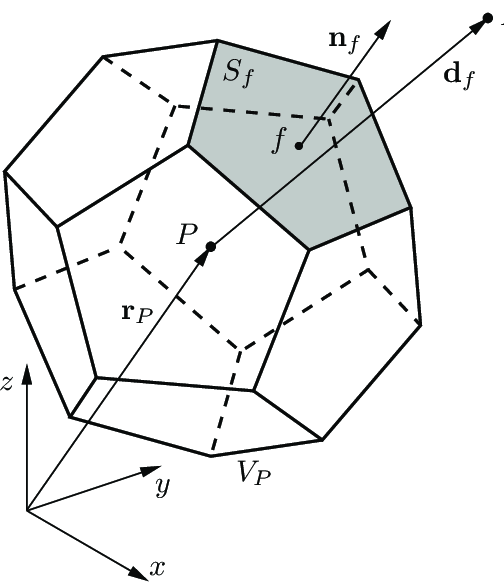
\includegraphics[width=0.8\linewidth]{Report/images/polycell.png}
    \caption{A typical finite volume cell; with a general polyhedral shape. See \ref{tab:notation} for nomenclature. Image taken from \cite{Tukovic2018OpenfoamInteraction}.}
    \label{fig:polycell}
\end{figure}
\begin{itemize}

    \item they must be convex in shape, that is, the angle between the face normal, $\mathbf{n}_f$, and the delta vector, $\mathbf{d}_f = \overline{PN}$, should not exceed $90^{\circ}$, where $\overline{PN}$ is the vector between the centroids of cells $P$ and $N$, neighbouring cell.
    \item each cell $P$ can share at most one face with a neighbouring cell $N$;
    \item each face $f$ has an owner cell and a neighbour cell, defined by the direction of the face normal vector $\mathbf{n}_f$. The normal always points into the owner cell, mathematically $\mathbf{n}_f \cdot \mathbf{d}_f < 0$. The left-hand rule convention is used to define the direction of the face normal vector, always pointing \textit{out} of the owner cell;gT
    \item faces that lie within the domain, having both an owner and a neighbour, are called \textit{internal faces}. While faces that lie on the domain boundary, having only an owner face, are called \textit{boundary faces};
    \item finally, the cell and face centroids are defined mathematically as $$\int_{V_P} (\mathbf{x} - \mathbf{x}_P) dV = \mathbf{0}$$ and $$\int_{S_f} (\mathbf{x} - \mathbf{x}_f) dS = \mathbf{0}$$ respectively;
    \item finally, second-order variation of dependent variables in space and time is assumed to obtain a second-order accurate discretisation method, i.e. for some scalar $\phi$, such as $v_x$ or $p$, 
    \begin{gather}
        \phi(\mathbf{x}) = \phi _P + (\mathbf{x} - \mathbf{x}_P) \cdot (\nabla \phi)_P
        \label{eqn:spatial_recon}
        \\
        \phi(t+\Delta t) = \phi ^t + \Delta t \left(\frac{\partial \phi}{\partial t}\right)_t
        \label{eqn:temporal_recon}
    \end{gather}
    
\end{itemize}


\subsection{The Governing Equations}
The equations governing the problem solved in this study are the \textit{incompressible Navier-Stokes equations} (\ref{eqn:INS_mass}) and (\ref{eqn:INS_momentum}).
To study the behaviour of this set of PDEs, it is necessary to integrate each equation over the CVs defined above. The solution of each dependent variable can be found in each CV, in line with the collocated arrangement discussed earlier. The task then is to integrate over an arbitrary cell volume, $V_P$, and over a time step, $\Delta t$, giving:

\begin{gather}
    \int_{V_P} (\nabla \cdot \mathbf{v}) dV = 0
    \label{eqn:continuity}
    \\
    \begin{split}
        &\int_{t}^{t+\Delta t} \biggl[ \frac{\partial}{\partial t} \int_{V_P} \mathbf{v} dV + \int_{V_P} \nabla \cdot (\mathbf{v} \mathbf{v}) dV 
        \\
        - &\int_{V_P} \nabla \cdot (\nu \nabla \mathbf{v}) dV \biggr] dt = 
        - \int_{t}^{t+\Delta t} \biggl[\int_{V_P} \biggl( \nabla p + \mathbf{g} \biggr) dV \biggr] dt
    \end{split}
    \label{eqn:momentum}
\end{gather}

For this study, a few assumptions are made to simplify the equations further. Firstly, the problem is assumed to be steady-state so that any temporal derivatives can be ignored, and the integrals over time vanish. Secondly, the effect of gravity is neglected, removing the gravitational source term from the momentum equation. What remains is the dramatically simplified momentum equation, comprised of only \textit{Convection}, \textit{Diffusion}, and \textit{Source} terms:

\begin{gather}
    \underbrace{\int_{V_P} \nabla \cdot (\mathbf{v} \mathbf{v}) dV}_\textrm{Convection} - \underbrace{\int_{V_P} \nabla \cdot (\nu \nabla \mathbf{v}) dV}_\textrm{Diffusion} = - \underbrace{\int_{V_P} (\nabla p) dV}_\textrm{Source}
    \label{eqn:momentum_simp}
\end{gather}

To solve this system of equations implicitly, a matrix will be constructed to represent their integral form. For example, for some scaler variable $\phi$, the solution of the discretised PDE represents the value of $\phi$ at the centre of each finite-volume cell in the domain. Choosing some cell $P$, the cell-centred value of $\phi$ in $P$ is written $\phi _P$. Similarly, for cells neighbouring $P$, namely $N$, have cell-centred values of $\phi$ written $\phi _N$. The linear system can be written as a set of linear equations of the form $$a_P \phi_P + \sum \limits _N a_N \phi _N = b_P$$ where $a_P$, $a_N$, and $b_P$ represent matrix contributions in the diagonal, off-diagonal, and source terms respectively. Intuitively, $a_P$ is the mathematical representation of cell $P$'s effect on itself; $a_N$ of the $P$-$N$ interaction (in the upper triangle of the matrix) and the $N$-$P$ interaction (in the lower triangle); and $b_P$ of source effects in cell $P$. 

As a digression, the iterative method used to decouple pressure and velocity will be outlined before continuing with the details of constructing these matrix contributions. The resulting forms of the \textit{momentum} and \textit{continuity} equations will inform the discretisation thereof. 

\section{The SIMPLE Algorithm}
An acronym standing for \textbf{S}emi-\textbf{I}mplicit \textbf{M}ethod for \textbf{P}ressure \textbf{L}inked \textbf{E}quations \cite{Patankar1972AFLOWS}, the algorithm iteratively solves the momentum and continuity equations until convergence is reached. Since the algorithm aims to overcome the pressure-velocity coupling in the momentum equation, it begins naturally with a decoupling step. The initial pressure field in the discretised domain is guessed and used to solve the momentum equation. The resulting velocity field is unphysical since it was constructed from a likely unphysical pressure field. The continuity equation imposes a divergence-free constraint on the velocity field. Therefore, it can be used to calculate a pressure field that, in turn, is used to correct the velocities. However, the continuity equation in the form described above (\ref{eqn:continuity}) does not contain pressure; it will have to be manipulated into the pressure equation. Once the steps mentioned above have been completed, the procedure is cycled until the fields converge. \\ Here are the steps, in detail,

\begin{enumerate}
    \item Discretise the steady-state momentum equation, 
    \begin{equation}
        \nabla \cdot (\mathbf{v} \mathbf{v}) - \nabla \cdot (\nu \nabla \mathbf{v}) = 0
        \label{eqn:momentum_disc}
    \end{equation}
     In this study, the pressure gradient source term is omitted, and the divergence-free velocity corrections are done explicitly at the end of each iteration. Here, the velocity field is under-relaxed implicitly, as will be described shortly.
    \item Solve the discretised momentum equation implicitly with an iterative linear solver. The resulting velocity field will not be divergence-free.
    \item Assemble the face fluxes, the velocity flux through each finite-volume face in the domain, 
    \begin{equation}
        F_{pre} = \mathbf{s}_f \cdot \mathbf{v}_f ,
        \label{eqn:face_pre}
    \end{equation}
    where the cell-centred velocities, $\mathbf{v}_P$ and $\mathbf{v}_N$, are linearly interpolated to the face-centred velocity, $\mathbf{v}_f$, using (\ref{eqn:spatial_recon}) at the faces, 
    \begin{equation}
        \mathbf{v}_f = f_x \mathbf{v}_P + (1-f_x) \mathbf{v}_N ,
        \label{eqn:v_face}
    \end{equation}
    where $f_x = \overline{fN}/\overline{PN}$ is the ratio between face-neighbour and cell-neighbour distances.
    \item Discretise the pressure equation, consisting of the pressure Laplacian treated in the same manner as the momentum Laplacian term, and the flux divergence source term:
    \begin{equation}
        \nabla \cdot \left( \frac{1}{a_P} \nabla p \right) = \nabla \cdot \mathbf{v} ,
        \label{eqn:pressure_corr}
    \end{equation}
    calculated from $F_{pre}$.
    \item Construct divergence-free velocities at the faces and in the cell centres, using the corrected pressure and explicit under-relaxation:
    \begin{equation}
        F_{corr} = F_{pre} - \left( \frac{1}{a_P} \right)_f \mathbf{s}_f  \cdot (\nabla p)_f ,
        \label{eqn:flux_corr}
    \end{equation}
    and,
    \begin{equation}
        \mathbf{v}_{corr} = \mathbf{v}_{pre} - \frac{1}{a_P} \nabla p^{**}, 
        \label{eqn:velocity_corr}
    \end{equation}
    where pressure is under-relaxed via $$p^{**} = p^* - \alpha _p (p-p^*)$$
\end{enumerate}

\section{Matrix Construction}
\label{sec:matrix_constuction}

Returning to the finite volume discretisation of the governing equations, the task will be to calculate matrix coefficients $a_P$, $a_N$, and $b_P$ for each term in equations (\ref{eqn:momentum_disc}) and (\ref{eqn:pressure_corr}). 

\subsection{Convection Term}

The non-linear convection term, $\nabla \cdot (\mathbf{v v})$, has several competing ideas on dealing with it. In this study, the term will be linearised first and subsequently solved with a linear solver, whereas another method might be to use a solver for non-linear systems. \\
To linearise the convection term, the product, $(\mathbf{v v})$, is split into a \textit{convecting} velocity, $\mathbf{v}^o$, and a \textit{convected} velocity, $\mathbf{v}^n$. Therefore, the scheme is not strictly implicit since $\mathbf{v}^o$ is the old velocity field. The convection term is then rewritten as $\nabla \cdot (\mathbf{v}^0 \mathbf{v}^n)$, and this is the form that is discretised. \\ 
Firstly, using Gauss' theorem (\ref{eqn:gauss3}) and the linear variation $\phi$ (\ref{eqn:spatial_recon}), choosing $\phi = v_x$ the x-velocity, it follows:

\begin{align}
    \begin{split}
        \int_{V_P} \nabla \cdot ( \mathbf{v}^o v_x^n ) dV &= \oint_{\partial V_P} (d\mathbf{S} \cdot \mathbf{v}^o ) v_x^n
        \\
        &= \sum\limits_f \Biggl( \int_f (d\mathbf{S} \cdot \mathbf{v}^o) v_x^n \Biggr)
        \\ 
        &= \sum\limits_f \Biggl[ \biggl( \int_f (d\mathbf{S} \Biggr) \cdot \mathbf{v}^o
        \\
        &+ \Biggl( \int_f d\mathbf{S} (\mathbf{x} - \mathbf{x}_f) \Biggr) \cdot (\nabla \mathbf{v}^o)_f \Biggr]  v_x^n 
        \\
        &= \sum\limits_f (\mathbf{S} \cdot \mathbf{v}^o) v_x^n
        \\
        &= \sum\limits_f F (v_x^n)_f
    \end{split}
\end{align}
where $F$ is the flux through face $f$: $$F = \mathbf{S} \cdot (\mathbf{v}^o)_f$$
\\ 
The next task is to determine the face centroid value of the connecting velocity, $\mathbf{v}^o$. A differencing scheme is a method in which the value at the face is determined as a combination of the cell values on either side of the face. Since the finite volume mesh is not structured in any predictable way, it is not practical to use any values besides those adjacent to the face itself, namely $\mathbf{v}_P$ and $\mathbf{v}N$. In this study, \textit{Upwind differencing} is used. Given that the connecting velocity has a direction, it is clear which direction the information it is transporting is coming from and going towards. Therefore, the face-centred value is simply the cell-centred value of the cell from which information is travelling, the upwind cell. Mathematically, this reads,
\begin{equation}
    \mathbf{v}_f = 
    \begin{cases}
          \mathbf{v}_P & \text{for} F \geq 0 ,\\
          \mathbf{v}_N & \text{for} F < 0 .
    \end{cases}
    \label{eqn:upwind_diff}
\end{equation}

While this scheme guarantees that spurious oscillations do not form and the solution is bounded, it also introduces significant numerical diffusion, violating the order of accuracy of the solution. \\ 
The matrix contributions, therefore, are as follows:
\begin{align}
    \label{eqn:conv_matrix}
    &a_P = max(F , 0) , \\
    &a_N = min(F , 0) .
\end{align}

\subsection{Laplacian Term}
Both the momentum and the pressure equations have a Laplacian term, i.e. the divergence of the gradient of a field. In the momentum equation (\ref{eqn:momentum_disc}) there is the Diffusion term, $- \nabla \cdot (\nu \nabla \mathbf{v})$, and in the pressure equation (\ref{eqn:pressure_corr}) there is the Pressure Laplacian, $\nabla \cdot 1/a_P \nabla p $. Both of these terms have the same form and will therefore be discretised identically from the general form, 
\begin{equation}
    \label{eqn:laplacian}
    \underbrace{\nabla \cdot \mu \nabla \phi}_\textrm{Laplacian}    
\end{equation}
In a similar manner to the convection term above, the Laplacian is discretised using the assumption of linear variation of $\phi$ and using Gauss' theorem, giving
\begin{align}
    \begin{split}
        \int_{V_P} \nabla \cdot (  \mu \nabla \phi  ) dV &= \sum\limits_f \mathbf{S} \cdot (  \mu \nabla \phi )_f
        \\
        &= \sum\limits_f (\mu)_f \mathbf{S} \cdot ( \nabla \phi )_f .
    \end{split}
    \label{eqn:laplacian_simplif}
\end{align}
In this study, it is assumed that the mesh is orthogonal, which is generally not true. In fact, orthogonality is more of an exception than a rule for unstructured meshes. Nevertheless, its existence provides simplicity in computing the Laplacian term. Vectors $\mathbf{d}$ and $\mathbf{S}_f$ are parallel in an orthogonal mesh, giving the following:
\begin{equation}
    \label{eqn:laplac_SgradPhi}
    \mathbf{S} \cdot (\nabla \phi)_f = |\mathbf{S}| \frac{\phi_N - \phi_P}{|\mathbf{d}|}.
\end{equation}
Which, along with (\ref{eqn:laplacian_simplif}), and summing over all faces in a cell $P$, results in the matrix coefficients:
\begin{align}
    \label{eqn:lapl_matrix}
    &a_P = - \sum\limits_f \mu |\mathbf{S}_f| \delta_f , \\
    &a_N = \mu |\mathbf{S}_f| \delta_f .
\end{align}
where $\delta_f = 1/|\mathbf{d}_f|$.

\subsection{Continuity Source Term}
The right-hand side of the pressure equation (\ref{eqn:pressure_corr}) contains a source term which is simply the divergence of the velocity field, $\nabla \cdot \mathbf{v}$. Despite the fact that this term is supposed to sum to zero by the continuity constraint (\ref{eqn:continuity}), it contributes to the pressure correction since the velocity fields are not initially divergence-free. \\ As seen in the convection term discretisation, the divergence of the velocity field is given by: 
\begin{equation}
    \label{eqn:laplac_SgradPhi}
    \int_{V_P} (\nabla \cdot \phi)dV = \sum\limits _f F
\end{equation}
which is calculated from the velocity field solution of the momentum equation. \\ In terms of matrix contributions, the sum over all internal faces adds to owner and neighbour source terms,
\begin{align}
    \label{eqn:conv_matrix}
    &b_P = F & \text{for all cells,}\\
    &b_N = -F & \text{for all internal cells}.
\end{align}

\subsection{Boundary Conditions}
In the case of control volumes on the finite-volume domain's boundary, the governing equation's discretisation differs. This is due to the fact that faces on the boundary only have an owner cell since the neighbour would be outside the domain. As a result, the practice numerically prescribes the conditions at the boundary. This is done in several ways, either by prescribing the \textit{value} of a variable at the boundary face, known as \textbf{Dirichlet} or \textbf{Fixed Value} boundary conditions or by prescribing the \textit{gradient} of a variable at the boundary face, known as \textbf{Von Neumann} or \textbf{Fixed Gradient} boundary conditions. A third option exists, in which a combination of the two is used, called \textbf{Mixed} boundary conditions. \\
The boundary condition discretisation for the momentum and pressure equations are then given by:

\begin{itemize}
    \item \textbf{Dirichlet Boundary Condition} \\
        As described above, the fixed-value boundary condition prescribes the value of a variable at the boundary face $b$. The convection, Laplacian, and continuity terms need to take this into account: 
        \begin{itemize}
            \item \textbf{Convection term}. Here the boundary face velocity $\mathbf{v}_b$ is prescribed, giving a source term contribution in the momentum equation discretisation:
            \begin{equation}
                \label{eqn:diri_bc_conv}
                b_P = F_b (v_x)_b ,
            \end{equation}
            where $F_b$ is the boundary face flux calculated with the fixed value boundary velocity from the previous iteration (if these are non-constant).

            \item \textbf{Laplacian term}. Here the boundary value of $\phi$ is given as $\phi_b$, resulting in
            \begin{equation}
                \label{eqn:laplac_bc_SgradPhi}
                \mathbf{S} \cdot (\nabla \phi)_b = |\mathbf{S}| \frac{\phi_b - \phi_P}{|\mathbf{d}|}.
            \end{equation}
            which gives the same diagonal matrix contribution but additionally gives a source term: 
            \begin{align}
                \label{eqn:lapl_bc_matrix}
                &a_P = - \mu |\mathbf{S}_b| \delta_b , \\
                &b_P = - \mu |\mathbf{S}_b| \delta_b \phi_b.
            \end{align}
            \item \textbf{Continuity source term}. Finally, the fixed value boundary condition adds a fixed face flux contribution to the pressure equation source: 
            \begin{align}
                \label{eqn:conv_matrix}
                b_P = F_b
            \end{align}
        \end{itemize}
    \item \textbf{Von Neumann Boundary Condition} \\
    The fixed-gradient boundary condition prescribes the gradient of a variable at the boundary face centre, $g_b$. The convection and laplacian terms need to take this into account:
    \begin{itemize}
            \item \textbf{Convection term}. Here the boundary face velocity gradient $(\nabla \mathbf{v})_b$ is prescribed. The boundary face velocity is then calculated from the cell centre value and this gradient, giving a source term contribution:
            \begin{equation}
                \label{eqn:neu_bc_conv}
                b_P = F_b (v_x)_b ,
            \end{equation}
            where
            \begin{equation}
                F_b = \mathbf{S}_b \cdot \bigl(\mathbf{v}_P + \mathbf{d}_b \cdot \mathbf{v}_b \bigr) ,
            \end{equation}
            and
            \begin{equation}
                (v_x)_b = (S_x)_b \bigl((v_x)_P + (d_x)_b (v_x)_b \bigr)
            \end{equation}

            \item \textbf{Laplacian term}. Here the boundary gradient of $\phi$ is given as $(\nabla \phi)_b$, which can be used directly in the calculation:
            \begin{align}
                \label{eqn:lapl_bc_matrix}
                &b_P = - \mu \mathbf{S}_b \cdot (\nabla \phi)_b.
            \end{align}
        \end{itemize}
\end{itemize}

\section{The Lid-Driven Cavity}
The specific problem simulated in this study is that of the benchmark fluid dynamics lid-driven cavity test from Ghia et al. \cite{Ghia1982High-ReMethod}. This is a 2-dimension simulation case involving a square, regular Cartesian domain with a fixed velocity boundary condition along the top edge (See Figure \ref{fig:lid-driven}). The 2D square cavity has dimensions $0.1$m x $0.1$m, divided into $40$ x $40$ 2D, finite-volume cells. A 2D finite-volume cell is treated as a 3D unstructured cell in which the depth of the domain is defined arbitrarily and ignored in the simulation, except when using the face area (In reality, this depth does not affect the outcome of the simulation; it simply scales the calculations by a constant amount).
\begin{figure}[ht]
    \centering
    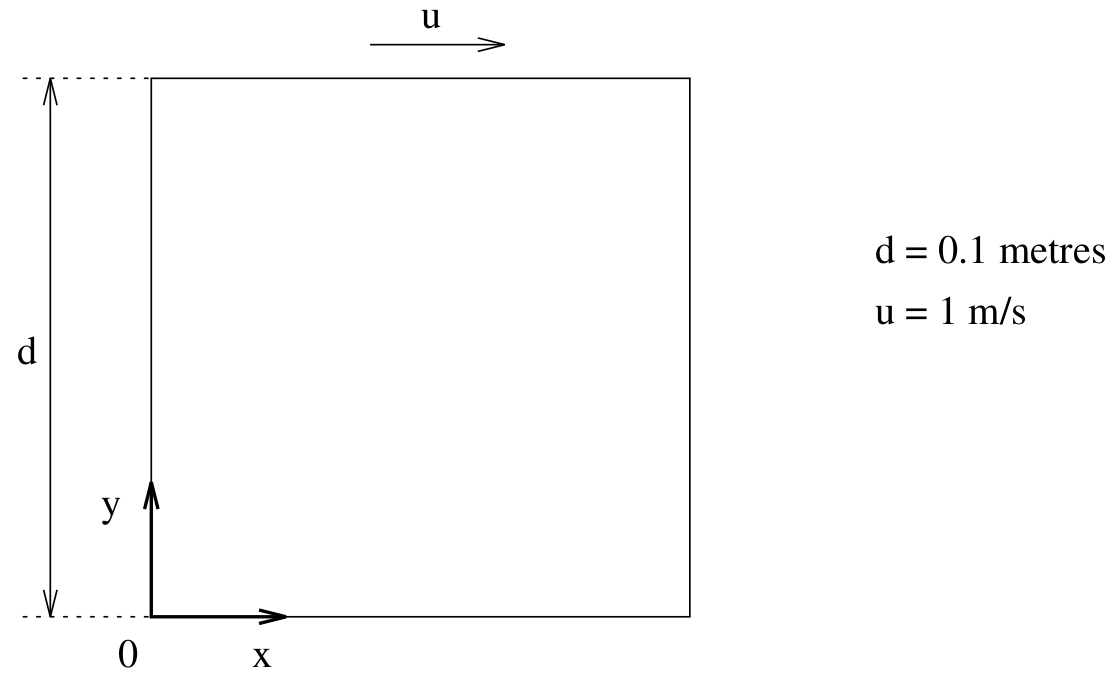
\includegraphics[width=\linewidth]{Report/images/lid-driven-cavity.png}
    \caption{The lid-driven cavity domain, with fixed value velocity along the top edge of $\mathbf{v} = (1,0)$. }
    \label{fig:lid-driven}
\end{figure}

The simulation will involve solving the steady-state incompressible Navier-Stokes equations for laminar flow and implementing the SIMPLE algorithm for pressure-velocity coupling. The simulation case is set up as follows:
\begin{itemize}
    \item Dirichlet boundary conditions on velocity, $\mathbf{v}$, on all sides:
    \begin{itemize}
        \item $\mathbf{v}_b = (1,0)$m/s along the top (lid) boundary.
        \item $\mathbf{v}_b = (0,0)$m/s on all other sides.
    \end{itemize}
    \item Von Neumann boundary conditions on pressure gradient, $(\nabla p)_b = (0,0)$m$^2$/s, on all sides.
    \item Reynolds number $Re = 100$, defining the kinematic viscosity over the whole domain.
\end{itemize}
convert eps to pdf ubuntu
\section{Code Structure}
This section will give a high-level outline of the code written to run the simulation (See README for cloning and testing of code). \\ The simulation is split into three separate parts: the unstructured finite-volume mesh for discretised space, \texttt{fvMesh} class and associated classes, the finite-volume matrix for discretised equations, \texttt{fvMatrix}, and finally, the simulation and SIMPLE algorithm, \texttt{fvSimulation} and \texttt{SIMPLE}. 

\subsection{Finite-Volume Mesh Class}
The discretisation of the spatial domain is implemented through the \texttt{fvMesh} class which facilitates the creation and storage of an unstructured mesh. A partial description of the class will be given here to highlight the important parts of its functioning. The class is composed of the following member variables and helper classes:
\begin{itemize}
    \item An array of \texttt{points}.
        \begin{itemize}
            \item Each \texttt{point} is a three-dimensional array of doubles.
        \end{itemize}
    \item An array of \texttt{Face} objects.
        \begin{itemize}
            \item Each face is made up of a set of indices in the \texttt{point} array, 
            \item Each face has a \texttt{face centroid}, $f$, a \texttt{face area vector}, $\mathbf{S}_f$, and a \texttt{delta} value, $\delta_f = 1/|\mathbf{d}_f|$. 
        \end{itemize}
    \item An array of \texttt{Cell} objects.
        \begin{itemize}
            \item Each cell is made up of a set of indices in the \texttt{Face} array, 
            \item Each cell has a \texttt{cell centroid}, $P$, and a \texttt{cell volume}, $\mathbf{V}_P$.
        \end{itemize}
    \item An array of \texttt{BoundaryPatch} objects.
        \begin{itemize}
            \item Each boundary patch comprises a start \texttt{Face} index, a number of faces, and a patch name. 
            \item Each boundary patch object will also store the patch type (e.g. \texttt{fixedValue} or \texttt{fixedGrad}) and a value, such as $\mathbf{v}_b$.
        \end{itemize}convert eps to pdf ubuntu
\end{itemize}
 Additionally, \texttt{fvMeshParser} is used to import and create the \texttt{fvMesh} from the output of the \texttt{OpenFOAM blockMesh} utility, and \texttt{VectorUtils} is used to simplify the calculation of face areas and cell volumes by tesselation. 

 \subsection{Finite-Volume Matrix Class}
 The discretisation of the momentum and pressure equations is done using the \texttt{fvMatrix} class which facilitates the creation and linear solving of these equations. The data structures used to store the matrix, $\mathbf{A}$ and the column vectors of solutions and sources, $\mathbf{b}$, are created using the \texttt{Armadillo} library  \cite{Cubasch2010Armadillo:Experiments}. Matrices are stored in the dense matrix format with \texttt{arma::mat} and column vectors with \texttt{arma::vec}. The linear system is solved using the \texttt{arma::solve} function (For more on this, see Cubasch \cite{Cubasch2010Armadillo:Experiments})\footnote{This choice of dense format storage and library solver was due to time constraints. Ideally, a self-implemented sparse format data structure and Gauss-Seidel linear solver}. 
 The remaining details of the implementation of the \texttt{fvMatrix} class are as follows:
\begin{itemize}
    \item Discretisation of the aforementioned PDE terms (Section \ref{sec:matrix_constuction}). 
        \begin{itemize}
            \item \texttt{discretizeConvectionUpwind} for the convection term.
            \item \texttt{discretizeLaplacian} for both the momentum and pressure equation Laplacian terms.
            \item \texttt{discretizeContinuity} for the pressure equation continuity source term.
        \end{itemize}
    \item Since the discretisation of $a_P$ and $a_N$ is identical for both $v_x$ and $v_y$, but the source terms are different, two source column vectors are stored, \texttt{bx} and \texttt{by}. 
    \item The system is then solved separately by calling \texttt{solveLinearSystem} parsing a \texttt{bool} value to determine the dimension being solved (\texttt{true} for solving with \texttt{bx}, \texttt{false} for solving with \texttt{by}).
\end{itemize}

\subsection{SIMPLE Algorithm Simulation Class}
Finally, the classes responsible for the execution of the simulation are \texttt{fvSimulation} and \texttt{SIMPLE}. They work in tandem do the following:
\begin{itemize}
    \item Create a \texttt{fvMesh} object from the \texttt{blockMesh} files.
    \item Initialize vector field, $\mathbf{v}$, and scalar field, $p$.
    \item Execute all steps in the SIMPLE algorithm, including:
    \begin{itemize}
        \item \texttt{calculateFluxes} from the velocity field.
        \item Discretise and solve the momentum equation.
        \item Discretise and solve the pressure equation.
        \item Assemble conservative face fluxes \texttt{correctF} and divergence-free velocity field \texttt{correctU}.
    \end{itemize}
\end{itemize}

\section{Results and Discussion}
This section will present the results of the lid-driven cavity simulation using the finite-volume method and the steady-state incompressible Navier-Stokes equations. 

Firstly, the simulation is run four times, each with a different number of SIMPLE algorithm iterations, 1, 5, 10, and 20, respectively. \\ In each iteration, the $F_{pre}$ and $F_{corr}$ are printed. $F_{pre}$ shows that the momentum equation produces a velocity field that is not divergence-free, while $F_{corr}$ shows that the pressure equation gives a pressure field that can be used to construct the divergence-free velocity field. As an example, Figure \ref{fig:divU} is the output after the first SIMPLE iteration.

\begin{figure}[ht]
    \centering
    \fbox{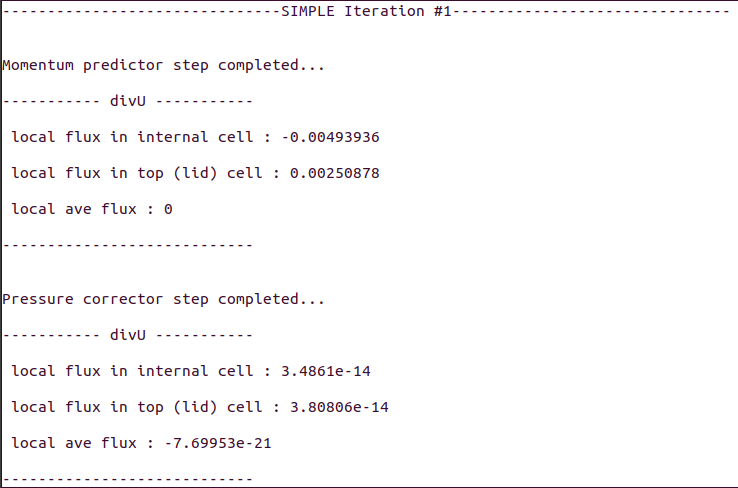
\includegraphics[width=\linewidth]{Report/images/divU.png}}
    \caption{A comparison of the local (cell) sum of $F$ before and after the pressure corrector step of the algorithm.}
    \label{fig:divU}
\end{figure}

Secondly, to ensure that the discretisation of the momentum and pressure equations are as expected, the diagonal ($a_P$), off-diagonal ($a_N$), and source ($b_x$ and $b_y$) contributions are reported for the first iteration of the SIMPLE algorithm in Figure \ref{fig:mat_coeff}.

\begin{figure}[ht]
    \centering
    \fbox{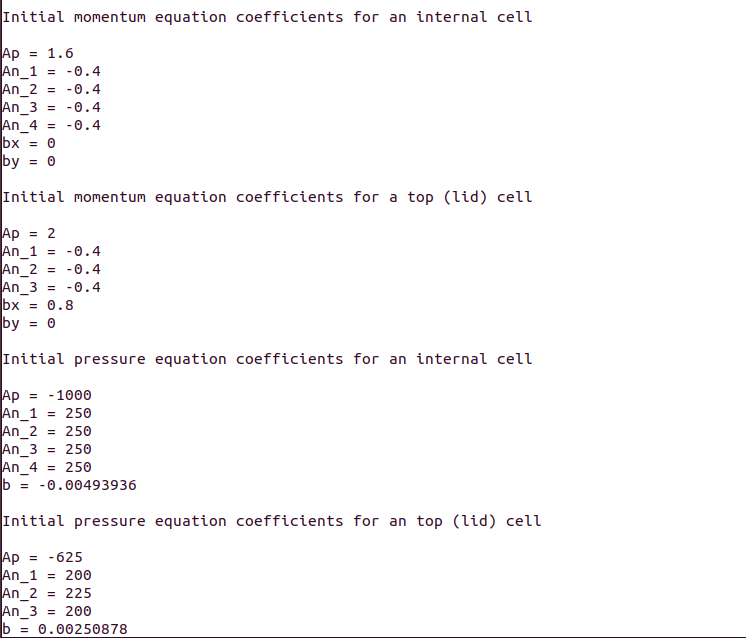
\includegraphics[width=\linewidth]{Report/images/mat_coeffs.png}}
    \caption{Matrix coefficients of momentum and pressure equation discretisation for the first iteration of the SIMPLE algorithm, }
    \label{fig:mat_coeff}
\end{figure}

Finally, the system is visualized after 1 iteration (Figure \ref{fig:1iter}) and after 20 iterations (Figure \ref{fig:20iter}). In both cases, a clear vortex is present in the upper-right of the cavity, with the velocity field carrying fluid in a clockwise direction as expected from a right-moving lid. The only noticeable difference between the two cases is the exact position of the centre of the vortex, where in Figure \ref{fig:1iter} it is centred at approximately $(0.5, 0.6)$, in Figure \ref{fig:20iter} it has shifted to approximately $(0.6, 0.7)$

\begin{figure}[ht]
    \centering
    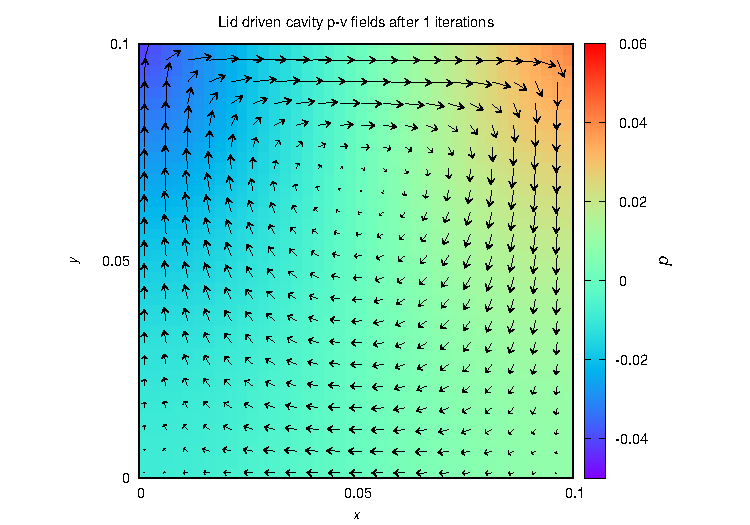
\includegraphics[width=\linewidth]{Report/images/1.pdf}
    \caption{Lid-driven cavity pressure-velocity solution after 1 SIMPLE iteration. $Re=100$. }
    \label{fig:1iter}
\end{figure}

\begin{figure}[ht]
    \centering
    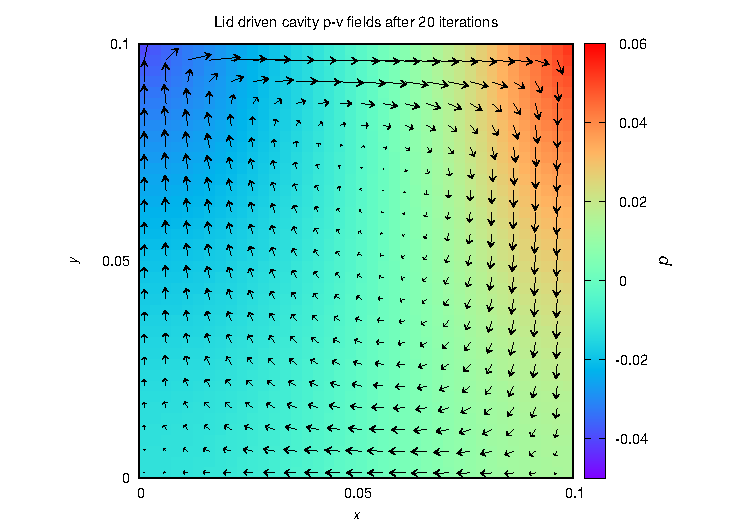
\includegraphics[width=\linewidth]{Report/images/20.pdf}
    \caption{Lid-driven cavity pressure-velocity solution after 20 SIMPLE iterations. $Re=100$.}
    \label{fig:20iter}
\end{figure}

The lid-driven cavity problem is a fundamental problem in fluid mechanics that has been used as a benchmark to test various numerical methods. One important parameter in this method is the under-relaxation factor, which controls how much the computed solution is updated at each iteration. If the under-relaxation factor is too low, the solution may converge slowly, while a too high value may lead to oscillations or even divergence in the solution. In this case, under-relaxation was not used, which means that the computed solution is updated with the full value of the computed velocity and pressure fields at each iteration.

The results of the solution to the lid-driven cavity problem with pressure-velocity coupling and the SIMPLE algorithm can be seen in Figures \ref{fig:1iter} and \ref{fig:20iter}, and showed that the solution appeared very similar after one iteration and after twenty iterations. This suggests that the solution has already converged to a steady state after the first iteration. This is surprising because it is generally expected that the solution will require many iterations to reach a steady state, especially is cases where under-relaxation is not used. However, it is important to note that this rapid convergence may be due to the initial conditions and the chosen parameters. 

When compared to the results from a similar investigation \cite{StracciaA2018HowBlog}, the steady-state solution seems satisfactory.

\section{Conclusion and Future Work}
This MPhil assignment implemented an unstructured Finite-Volume mesh class according to Peric \cite{Peric1985ADucts.} and solved the benchmark lid-driven cavity \cite{Ghia1982High-ReMethod}. The steady-state solution involving pressure-velocity was found using 20 iterations of the SIMPLE algorithm \cite{Patankar1972AFLOWS}, where the steady-state incompressible Navier-Stokes were discretized by the standard finite-volume discretization of the Laplacian, convection, and continuity source term. The upwind convection differencing scheme was used for the convection discretization. \\ The solution appeared to converge to steady-state after just one iteration, as it appeared almost unchanged between 1 and 20 iterations. This is surprising since under-relaxation was not applied to the discretization, which classically is a necessary step to achieve convergence. 
%% ############################################################################################

%% The Appendices part is started with the command \appendix;
%% appendix sections are then done as normal sections
\appendix

\section{Notation, Symbols and Acronyms}
\label{app:notation}

\begin{table}[ht]
\caption{Table of nomenclature used in report}
\label{tab:notation}
\begin{tabular}{ll}
\hline
$t$               & time                     \\
$\rho$            & density                  \\
$\mathbf{v}$      & velocity                 \\
$P$               & pressure                 \\
$p$               & kinematic pressure       \\
$E$               & total energy             \\
$\mathbf{f}$      & external forces          \\
$\mathbf{\tau}$   & deviatoric stress tensor \\
$\nabla$ & nabla operator $(\frac{\partial}{\partial x}, \frac{\partial}{\partial y}, \frac{\partial}{\partial z}$) \\
$\mathbf{I}$      & identity matrix          \\
$\mathbf{\kappa}$ & thermal conductivity     \\
$\mathbf{g}$      & gravitational force      \\
$P$               & cell centroid            \\
$f$               & face centroid            \\
$V_P$             & cell volume              \\
$S_f$             & face area                \\
$\mathbf{n}_f$    & face normal vector       \\
$\mathbf{d}_f$    & face delta vector       
\end{tabular}
\end{table}

\section{Additional Mathematics}
\label{app:maths}
\subsection{Gauss' Theorem}

The generalised form of Gauss' theorem can be written as,
\begin{gather}
    \int_V \nabla \cdot \mathbf{a} dV = \oint_{\partial V} d\mathbf{S} \cdot \mathbf{a} , 
    \label{eqn:gauss1}
    \\
    \int_V \nabla \phi dV = \oint_{\partial V} d\mathbf{S} \phi , 
    \label{eqn:gauss2}
    \\
    \int_V \nabla \mathbf{a} dV = \oint_{\partial V} d\mathbf{S} \mathbf{a} , 
    \label{eqn:gauss3}
\end{gather}
where $\partial V$ is the surface bounding the arbitrary volume $V$, with $d\mathbf{S}$, an infinitesimal surface element.




%% References
%%
%% Following citation commands can be used in the body text:
%% Usage of \cite is as follows:
%%   \cite{key}         ==>>  [#]
%%   \cite[chap. 2]{key} ==>> [#, chap. 2]
%%

%% References with bibTeX database:

\newpage
\bibliographystyle{Report/elsarticle-num-nourl.bst}
\bibliography{Report/SIMPLE_Refs.bib}

%% Authors are advised to submit their bibtex database files. They are
%% requested to list a bibtex style file in the manuscript if they do
%% not want to use elsarticle-num.bst.

%% References without bibTeX database:

% \begin{thebibliography}{00}

%% \bibitem must have the following form:
%%   \bibitem{key}...
%%

% \bibitem{}

% \end{thebibliography}


\end{document}

%%
%% End of file `elsarticle-template-num.tex'.
